\documentclass[11pt, a4paper] {ncc}
\usepackage[utf8] {inputenc}
\usepackage[T2A]{fontenc}
\usepackage[english, russian] {babel}
\usepackage[usenames,dvipsnames]{xcolor}
\usepackage{listings,a4wide,longtable,amsmath,amsfonts,graphicx,tikz}
\usepackage{pgfplots}
\usepackage{indentfirst}
\usepackage{bytefield}
\usepackage{multirow}
\usepackage{tabularx}
\usepackage[left=1.5cm,right=1.5cm,top=2cm,bottom=1.5cm,bindingoffset=0cm]{geometry}

\begin{document}
\setcounter{figure}{0}
\frenchspacing
\pagestyle{empty}
\begin{center}
     Национальный исследовательский университет информационных технологий,
                              механики и оптики\\
                        Кафедра вычислительной техники\\
                          Сети ЭВМ и телекоммуникации
\end{center}
\vspace{\stretch{2}}
\begin{center}
                            Учебно-исследовательская работа №3\\
                        <<Основы администрирования маршрутизируюмых компьютерных сетей>>\\
                                Вариант 38
\end{center}
\vspace{\stretch{3}}
\begin{flushright}
                                          Студентка:\\
                                                         {\it Куклина М., P3301} \\
                                          Преподаватель:\\
                                                         {\it Шинкарук Д.Н. }
\end{flushright}
\vspace{\stretch{4}}
\begin{center}
                             Санкт-Петербург, 2017
\end{center}
\newpage


\section*{Цели работы}
    Изучение основных методов настройки маршрутизируемых компьютерных сетей на примере сети,
    состоящей из компьютеров под управлением ОС Linux.

\section*{Общая часть}
    \subsection*{Настройка сети}
        Для реализации вполне неоднозначного и запутанного задания была создана сеть из четырёх
        хостов, состоящих в одной внутренней сети.
        \begin{figure}[h!]
            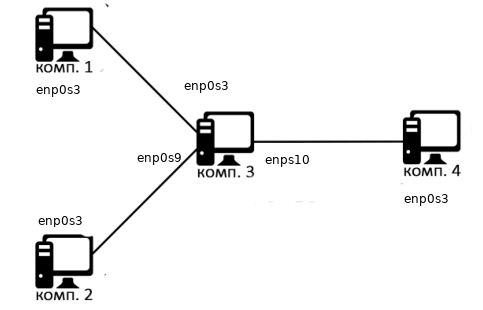
\includegraphics[scale=0.5]{./base.png}
        \end{figure}

        Для обеспечения сетевой доступности и выполнения задания пл iptables были 
        выполнены следующие действия.

        На шлюзе.
\begin{verbatim}
# Up interfaces.
    ip link set enp0s3 up
    ip link set enp0s9 up
    ip link set enp0s10 up

# Flush old ip addresses from all interfaces.
    ip a flush enp0s3
    ip a flush enp0s9
    ip a flush enp0s10
# Set new ip addresses for each interface.
    ip a add 5.7.1.3/24 dev enp0s3
    ip a add 5.7.2.3/24 dev enp0s9
    ip a add 5.7.4.3/24 dev enp0s10
# Enable ip routing.
    echo 1 > /proc/sys/net/ipv4/ip_forward
\end{verbatim}

    На хосте А.
\begin{verbatim}
    ip link set enp0s3 up
    ip a flush enp0s3
    ip a add 5.7.4.4/24 dev enp0s3
    ip r add default via 5.7.4.3
\end{verbatim}

    На хосте Б.
\begin{verbatim}
    ip link set enp0s3 up
    ip a flush enp0s3
    ip a add 5.7.2.2/24 dev enp0s3
    ip r add default via 5.7.2.3

\end{verbatim}

    На дополнительном хосте.
\begin{verbatim}
    ip link set enp0s3 up
    ip a flush enp0s3
    ip a add 5.7.1.1/24 dev enp0s3
    ip r add default via 5.7.1.3
\end{verbatim}

    Тесты.
    \begin{enumerate}
        \item ping \\
            Пингуется.
        \item nc \\
            Хост A: \texttt{nc -ulp 1337}\\
            Хост Б: \texttt{nc 5.7.4.4 1337 -u}\\
            Работает.
        \item iptables \\
            Хост А.
            \begin{verbatim}
    iptables -F
# 1)
    iptables -A OUTPUT -o enp0s3 -p tcp --dport 1337 -j REJECT
# 4)
#   iptables -A INPUT -i enp0s3 -d 5.7.4.4 -j REJECT --reject-with\
#           icmp-host-unreachable
# 5)
    iptables -A INPUT -i enp0s3 -p icmp -m length ! --length 0:1000 -m \
        ttl --ttl-lt 10 -j REJECT
    iptables -A OUTPUT -o enp0s3 -p icmp -m length ! --length 0:1000 -m \
        ttl --ttl-lt 10 -j REJECT
            \end{verbatim}
            Хост Б.
            \begin{verbatim}
    iptables -F
# 2)
    iptables -A INPUT -i enp0s3 -p udp --sport 1337 -j REJECT
# 3)
#   iptables -A OUTPUT -o enp0s3 -s 5.7.2.2 -j REJECT --reject-with \
         icmp-host-unreachable
            \end{verbatim}
            \begin{enumerate}
                \item Запрет на передачу пакетов, отправленных на tcp-порт.\\
                    Хост А: \texttt{nc 5.7.2.2 1337}. \\
                    Хост C: \texttt{nc -lp 1337} \\
                    {\it Хост А отваливается. \\}
                    Хост А: \texttt{nc 5.7.2.2 1337 -u}. \\
                    Хост C: \texttt{nc -ulp 1337} \\
                    {\it Коммуникация налажена. \\}
                \item Запрет на приём пакетов, отправленных с udp-порта. \\
                    Хост Б: \texttt{nc 5.7.1.1 1337 -u} \\
                    Хост С: \texttt{nc -ulp 1337}\\
                    {\it Б $\to$ С: OK.\\
                    С $\to$ Б: Connection refused.}\\
                    Хост Б: \texttt{nc 5.7.1.1 1338 -u} \\
                    Хост С: \texttt{nc -ulp 1338}\\
                    {\itБ $\to$ С: OK.\\
                    С $\to$ Б: OK.}
                \item Запрет на передачу пакетов, отправленных с компьютера Б.\\
                    Хост Б: \texttt{ping 5.7.1.3}\\
                    \textit{Destination Host Unreachable}
                \item Запрет на приём пакетов, отправленных на компьютер А.
                    Хост А: \texttt{nc 5.7.1.1 1488 -u} \\
                    Хост C: \texttt{nc -ulp 1488} \\
                    {\it A $\to$ C: ok \\
                         C $\to$ A: Connection refused
                    }
                \item Запрет на приём и отправку ICMP пакетов, размер которых больше 1000 байт, а TTL меньше 10. \\
                    Хост А: \texttt{ping -s 2000 -t 9 5.7.1.1} \\
                    {\it Destination Port Unreachable} \\
                    Хост А: \texttt{ping -s 200 -t 9 5.7.1.1} \\
                    {\it OK} \\
                    Хост Б: \texttt{ping -s 2000 -t 9 5.7.4.4} \\
                    {\it Destination Port Unreachable} \\
                    Хост Б: \texttt{ping -s 200 -t 9 5.7.4.4} \\
                    {\it OK} \\
            \end{enumerate}
    \end{enumerate}
    
\section*{V1: вариант 3}
    На компьютерах 1 и 2 запущены два nc-сервера. На компьютере 4 запущен nc-клиент, который
    осуществляет подключение к IP-адресу, который не представлен в сети. На
    компьютее 3 настроен DNAT и дублирование трафика таким образом, чтобы оба
    nc-сервера получали запросу от nc-клиента. Ответные сообщение от серверов
    приходят отбратно к клиенту. Клиент и серверы работают по протоколу UDP.

    \subsection*{Топология сети}
        \begin{figure}[h!]
            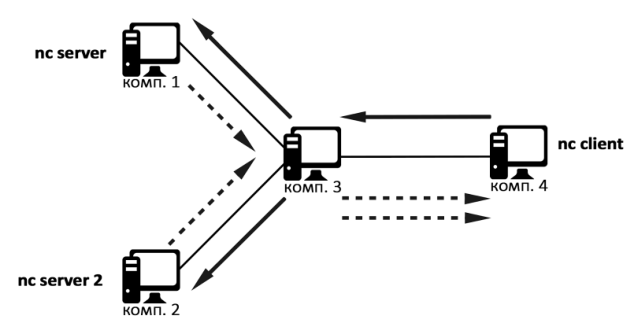
\includegraphics[scale=0.5]{v1_3.png}
            \caption{Топология сети и схема прохождения трафика}
        \end{figure}

    \subsection*{Настройка IPv4}
    Хост 1.
    \begin{verbatim}
  ip link set enp0s3 up
  ip addr flush dev enp0s3
  ip addr add 5.7.1.2/30 dev enp0s3
  ip route add default via 5.7.1.1
    \end{verbatim}
    Хост 2.
    \begin{verbatim}
  ip link set enp0s3 up
  ip addr flush dev enp0s3
  ip addr add 5.7.2.2/30 dev enp0s3
  ip route add default via 5.7.2.1
  iptables -t nat -F
  iptables -t nat -A PREROUTING -p udp -d 5.7.42.42 -j DNAT --to-dest 5.7.2.2
    \end{verbatim}
    Хост 3.
    \begin{verbatim}
  ip link set enp0s3 up
  ip link set enp0s9 up
  ip link set enp0s10 up
  ip addr flush dev enp0s3
  ip addr flush dev enp0s9
  ip addr flush dev enp0s10
  ip addr add 5.7.1.1/30 dev enp0s3
  ip addr add 5.7.2.1/30 dev enp0s9
  ip addr add 5.7.3.1/30 dev enp0s10
  echo 1 > /proc/sys/net/ipv4/ip_forward
  echo 0 | tee /proc/sys/net/ipv4/conf/*/rp_filter > /dev/null
  iptables -t nat -F
  iptables -t nat -A PREROUTING -i enp0s10 -d 5.7.42.42 -p udp \
                            -j DNAT --to-destination 5.7.1.2
  iptables -t nat -A POSTROUTING -d 5.7.3.2 -p udp \
                            -j SNAT --to-source 5.7.42.42
  iptables -t mangle -F
  iptables -t mangle -A PREROUTING -i enp0s10 -d 5.7.42.42 -p udp \
                            -j TEE --gateway 5.7.2.2
  iptables -t raw -F
  iptables -t raw -A PREROUTING -s 5.7.42.42 -p udp -j NOTRACK
    \end{verbatim}
    Хост 4.
    \begin{verbatim}
  ip link set enp0s3 up
  ip addr flush dev enp0s3
  ip addr add 5.7.3.2/30 dev enp0s3
  ip route add default via 5.7.3.1
    \end{verbatim}

    \subsection*{Настройка IPv6}
    Хост 1.
    \begin{verbatim}
  ip link set enp0s3 up
  ip -6 addr add ::ffff:5:7:1:2/126 dev enp0s3
  ip -6 route add default via ::ffff:5:7:1:1
    \end{verbatim}
    Хост 2.
    \begin{verbatim}
  ip link set enp0s3 up
  ip -6 addr add ::ffff:5:7:2:2/126 dev enp0s3
  ip -6 route add default via ::ffff:5:7:2:1
  ip6tables -t nat -F
  ip6tables -t nat -A PREROUTING -d ::ffff:5:7:9:9/128 -i enp0s3 -p udp \
                                -j DNAT --to-destination ::ffff:5:7:2:2
    \end{verbatim}
    Хост 3.
    \begin{verbatim}
  ip link set enp0s3 up
  ip link set enp0s9 up
  ip link set enp0s10 up
  ip -6 addr add ::ffff:5:7:1:1/126 dev enp0s3
  ip -6 addr add ::ffff:5:7:2:1/126 dev enp0s9
  ip -6 addr add ::ffff:5:7:3:1/126 dev enp0s10
  echo 1 | tee /proc/sys/net/ipv6/conf/*/forwarding > /dev/null
  echo 0 | tee /proc/sys/net/ipv6/conf/*/accept* > /dev/null
  ip6tables -t nat -F
  ip6tables -t nat -A PREROUTING -d ::ffff:5:7:9:9/128 -i enp0s10 -p udp \
                                 -j DNAT --to-destination ::ffff:5:7:1:2
  ip6tables -t nat -A POSTROUTING -d ::ffff:5:7:3:2/128 -p udp \
                            -j SNAT --to-source ::ffff:5:7:9:9
  ip6tables -t mangle -F
  ip6tables -t mangle -A PREROUTING -d ::ffff:5:7:9:9/128 -i enp0s10 -p udp \
                                             -j TEE --gateway ::ffff:5:7:2:2
  ip6tables -t raw -F
  ip6tables -t raw -A PREROUTING -s ::ffff:5:7:9:9 -p udp -j NOTRACK
    \end{verbatim}
    Хост 4.
    \begin{verbatim}
  ip link set enp0s3 up
  ip -6 addr add ::ffff:5:7:3:2/126 dev enp0s3
  ip -6 route add default via ::ffff:5:7:3:1
    \end{verbatim}


    TCP -- stateful протокол, ориентированный на установку соединений; протокол отслеживает состояние соединения
    и гарантирует целостность передаваемых данных, вследствие чего любые попытки установить связь с двумя
    серверами провалятся: пользовательский компьютер участвует во всех этапах соединения, 
    и он никогда не будет отвечать на два отдельных сервера, пытающихся связаться с ним.

\newpage
\section*{V2: вариант 8}

    \subsection*{Топология сети}
        \begin{figure}[h!]
            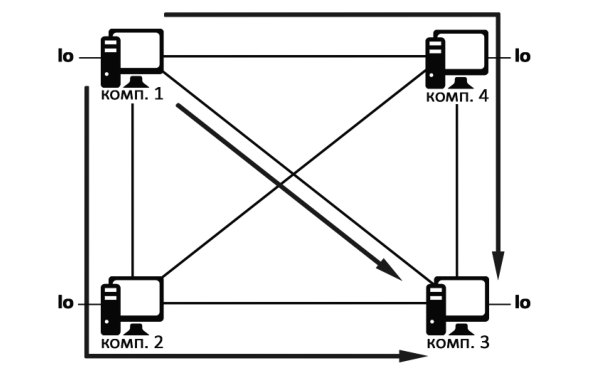
\includegraphics[scale=0.5]{lo.png}
            \caption{Топология сети и схема прохождения трафика}
        \end{figure}
    
    \subsection*{Настройка IPv4}
        \subsubsection*{Настройка хостов}
		Хост 1.
        \begin{verbatim}
          ip link set enp0s3 up
          ip link set enp0s9 up
          ip link set enp0s10 up

          ip addr add 5.7.1.1/24 dev enp0s3
          ip addr add 5.7.4.1/24 dev enp0s9
          ip addr add 5.7.6.1/24 dev enp0s10

          ip addr flush dev lo
          ip addr add 5.7.7.1/24 dev lo
         
          echo 0 | tee /proc/sys/net/ipv4/conf/*/rp_filter > /dev/null
          echo 1 > /proc/sys/net/ipv4/ip_forward
          echo 1 | tee /proc/sys/net/ipv4/conf/*/route_localnet>/dev/null
        \end{verbatim}
		Хост 2.
        \begin{verbatim}
          ip link set enp0s3 up
          ip link set enp0s9 up
          ip link set enp0s10 up

          ip addr add 5.7.2.2/24 dev enp0s3
          ip addr add 5.7.4.2/24 dev enp0s9
          ip addr add 5.7.5.2/24 dev enp0s10

          ip addr flush dev lo
          ip addr add 5.7.8.2/24 dev lo

          echo 0 | tee /proc/sys/net/ipv4/conf/*/rp_filter > /dev/null
          echo 1 > /proc/sys/net/ipv4/ip_forward
          echo 1 | tee /proc/sys/net/ipv4/conf/*/route_localnet>/dev/null
        \end{verbatim}
		Хост 3.
        \begin{verbatim}
          ip link set enp0s3 up
          ip link set enp0s9 up
          ip link set enp0s10 up

          ip addr add 5.7.1.3/24 dev enp0s3
          ip addr add 5.7.2.3/24 dev enp0s9
          ip addr add 5.7.3.3/24 dev enp0s10

          ip addr flush dev lo
          ip addr add 5.7.9.3/24 dev lo

          echo 0 | tee /proc/sys/net/ipv4/conf/*/rp_filter > /dev/null
          echo 1 > /proc/sys/net/ipv4/ip_forward
          echo 1 | tee /proc/sys/net/ipv4/conf/*/route_localnet>/dev/null
        \end{verbatim}
		Хост 4.
        \begin{verbatim}
          ip link set enp0s3 up
          ip link set enp0s9 up
          ip link set enp0s10 up

          ip addr add 5.7.3.4/24 dev enp0s3
          ip addr add 5.7.5.4/24 dev enp0s9
          ip addr add 5.7.6.4/24 dev enp0s10

          ip addr flush dev lo
          ip addr add 5.7.0.4/24 dev lo

          echo 1 > /proc/sys/net/ipv4/ip_forward
          echo 0 | tee /proc/sys/net/ipv4/conf/*/rp_filter > /dev/null
          echo 1 | tee /proc/sys/net/ipv4/conf/*/route_localnet >/dev/null
        \end{verbatim}

        \subsubsection*{Настройка маршрутов}
		Хост 1.
            \begin{verbatim}
    ip rule add prio 100 from 5.7.7.1 table 1
    ip r add 5.7.8.2 table 1 nexthop via 5.7.4.2 weight 1 \
                             nexthop via 5.7.1.3 weight 2 \
                             nexthop via 5.7.6.4 weight 3
    ip r add 5.7.9.3 table 1 nexthop via 5.7.4.2 weight 1 \
                             nexthop via 5.7.1.3 weight 2 \
                             nexthop via 5.7.6.4 weight 3
    ip r add 5.7.0.4 table 1 nexthop via 5.7.4.2 weight 1 \
                             nexthop via 5.7.1.3 weight 2 \
                             nexthop via 5.7.6.4 weight 3

    ip rule add prio 100 from 5.7.8.2 table 2
    ip r add 5.7.9.3 table 2 nexthop via 5.7.1.3 weight 2
    ip r add 5.7.0.4 table 2 nexthop via 5.7.4.2 weight 1

    ip rule add prio 100 from 5.7.9.3 table 3
    ip r add 5.7.8.2 table 3 nexthop via 5.7.4.2 weight 1
    ip r add 5.7.0.4 table 3 nexthop via 5.7.6.4 weight 3

    ip rule add prio 100 from 5.7.0.4 table 4
    ip r add 5.7.9.3 table 4 nexthop via 5.7.1.3 weight 2
    ip r add 5.7.8.2 table 4 nexthop via 5.7.4.2 weight 1
            \end{verbatim}
		Хост 2.
            \begin{verbatim}
    ip rule add prio 100 from 5.7.8.2 table 2
    ip r add 5.7.7.1 table 2 nexthop via 5.7.4.1 weight 1 \
                             nexthop via 5.7.2.3 weight 3 \
                             nexthop via 5.7.5.4 weight 2
    ip r add 5.7.9.3 table 2 nexthop via 5.7.4.1 weight 1 \
                             nexthop via 5.7.2.3 weight 3 \
                             nexthop via 5.7.5.4 weight 2
    ip r add 5.7.0.4 table 2 nexthop via 5.7.4.1 weight 1 \
                             nexthop via 5.7.2.3 weight 3 \
                             nexthop via 5.7.5.4 weight 2

    ip rule add prio 100 from 5.7.7.1 table 1
    ip r add 5.7.9.3 table 1 nexthop via 5.7.2.3 weight 3 
    ip r add 5.7.0.4 table 1 nexthop via 5.7.5.4 weight 2

    ip rule add prio 100 from 5.7.9.3 table 3
    ip r add 5.7.7.1 table 3 nexthop via 5.7.4.1 weight 1
    ip r add 5.7.0.4 table 3 nexthop via 5.7.5.4 weight 2

    ip rule add prio 100 from 5.7.0.4 table 4
    ip r add 5.7.7.1 table 4 nexthop via 5.7.4.1 weight 1
    ip r add 5.7.9.3 table 4 nexthop via 5.7.2.3 weight 3 
            \end{verbatim}
		Хост 3.
            \begin{verbatim}
    ip rule add prio 100 from 5.7.9.3 table 3
    ip r add 5.7.8.2 table 3 nexthop via 5.7.2.2 weight 3 \
                             nexthop via 5.7.1.1 weight 2 \
                             nexthop via 5.7.3.4 weight 1
    ip r add 5.7.7.1 table 3 nexthop via 5.7.2.2 weight 3 \
                             nexthop via 5.7.1.1 weight 2 \
                             nexthop via 5.7.3.4 weight 1
    ip r add 5.7.0.4 table 3 nexthop via 5.7.2.2 weight 3 \
                             nexthop via 5.7.1.1 weight 2 \
                             nexthop via 5.7.3.4 weight 1
   
    ip rule add prio 100 from 5.7.7.1 table 1
    ip r add 5.7.8.2 table 1 nexthop via 5.7.2.2 weight 3
    ip r add 5.7.0.4 table 1 nexthop via 5.7.3.4 weight 1

    ip rule add prio 100 from 5.7.8.2 table 2
    ip r add 5.7.7.1 table 2 nexthop via 5.7.1.1 weight 2
    ip r add 5.7.0.4 table 2 nexthop via 5.7.3.4 weight 1

    ip rule add prio 100 from 5.7.0.4 table 4
    ip r add 5.7.8.2 table 4 nexthop via 5.7.2.2 weight 3
    ip r add 5.7.7.1 table 4 nexthop via 5.7.1.1 weight 2
            \end{verbatim}
		Хост 4.
            \begin{verbatim}
    ip rule add prio 100 from 5.7.0.4 table 4
    ip r add 5.7.8.2 table 4 nexthop via 5.7.5.2 weight 2 \
                             nexthop via 5.7.3.3 weight 1 \
                             nexthop via 5.7.6.1 weight 3
    ip r add 5.7.9.3 table 4 nexthop via 5.7.5.2 weight 2 \
                             nexthop via 5.7.3.3 weight 1 \
                             nexthop via 5.7.6.1 weight 3
    ip r add 5.7.7.1 table 4 nexthop via 5.7.5.2 weight 2 \
                             nexthop via 5.7.3.3 weight 1 \
                             nexthop via 5.7.6.1 weight 3

    ip rule add prio 100 from 5.7.7.1 table 1
    ip r add 5.7.8.2 table 1 nexthop via 5.7.5.2 weight 2
    ip r add 5.7.9.3 table 1 nexthop via 5.7.3.3 weight 1

    ip rule add prio 100 from 5.7.8.2 table 2
    ip r add 5.7.9.3 table 2 nexthop via 5.7.3.3 weight 1
    ip r add 5.7.7.1 table 2 nexthop via 5.7.6.1 weight 3

    ip rule add prio 100 from 5.7.9.3 table 3
    ip r add 5.7.8.2 table 3 nexthop via 5.7.5.2 weight 3
    ip r add 5.7.7.1 table 3 nexthop via 5.7.6.1 weight 3
            \end{verbatim}

    \subsection*{Настройка IPv6}
        \subsubsection*{Настройка хостов}
		Хост 1.
\begin{verbatim}
  alias ip='ip -6'
  ip link set enp0s3 up
  ip link set enp0s9 up
  ip link set enp0s10 up

  ip addr add ::ffff:5:7:1:1/120 dev enp0s3
  ip addr add ::ffff:5:7:4:1/120 dev enp0s9
  ip addr add ::ffff:5:7:6:1/120 dev enp0s10

  ip addr add ::ffff:5:7:7:1/128 dev lo

  echo 1 | tee /proc/sys/net/ipv6/conf/*/forwarding > /dev/null
  echo 2 | tee /proc/sys/net/ipv6/conf/*/accept_ra > /dev/null

\end{verbatim}

	Хост 2.
\begin{verbatim}

  alias ip='ip -6'
  ip link set enp0s3 up
  ip link set enp0s9 up
  ip link set enp0s10 up

  ip addr add ::ffff:5:7:2:2/120 dev enp0s3
  ip addr add ::ffff:5:7:4:2/120 dev enp0s9
  ip addr add ::ffff:5:7:5:2/120 dev enp0s10

  ip addr add ::ffff:5:7:8:2/128 dev lo

  echo 1 | tee /proc/sys/net/ipv6/conf/*/forwarding > /dev/null
  echo 2 | tee /proc/sys/net/ipv6/conf/*/accept_ra > /dev/null

\end{verbatim}

	Хост 3.
\begin{verbatim}

  alias ip='ip -6'
  ip link set enp0s3 up
  ip link set enp0s9 up
  ip link set enp0s10 up

  ip addr add ::ffff:5:7:1:3/120 dev enp0s3
  ip addr add ::ffff:5:7:2:3/120 dev enp0s9
  ip addr add ::ffff:5:7:3:3/120 dev enp0s10

  ip addr add ::ffff:5:7:9:3/128 dev lo

  echo 1 | tee /proc/sys/net/ipv6/conf/*/forwarding > /dev/null
  echo 2 | tee /proc/sys/net/ipv6/conf/*/accept_ra > /dev/null
\end{verbatim}

	Хост 4.
\begin{verbatim}
  alias ip='ip -6'
  ip link set enp0s3 up
  ip link set enp0s9 up
  ip link set enp0s10 up

  ip addr add ::ffff:5:7:3:4/120 dev enp0s3
  ip addr add ::ffff:5:7:5:4/120 dev enp0s9
  ip addr add ::ffff:5:7:6:4/120 dev enp0s10

  ip addr add ::ffff:5:7:0:4/128 dev lo

  echo 1 | tee /proc/sys/net/ipv6/conf/*/forwarding > /dev/null
  echo 2 | tee /proc/sys/net/ipv6/conf/*/accept_ra > /dev/null

\end{verbatim}

        \subsubsection*{Настройка маршрутов}

\begin{verbatim}
  alias ip='ip -6'
    ip rule add prio 100 from ::ffff:5:7:7:1 table 1
    ip r add ::ffff:5:7:8:2 table 1 nexthop via ::ffff:5:7:4:2 weight 1 \
                             nexthop via ::ffff:5:7:1:3 weight 2 \
                             nexthop via ::ffff:5:7:6:4 weight 3
    ip r add ::ffff:5:7:9:3 table 1 nexthop via ::ffff:5:7:4:2 weight 1 \
                             nexthop via ::ffff:5:7:1:3 weight 2 \
                             nexthop via ::ffff:5:7:6:4 weight 3
    ip r add ::ffff:5:7:0:4 table 1 nexthop via ::ffff:5:7:4:2 weight 1 \
                             nexthop via ::ffff:5:7:1:3 weight 2 \
                             nexthop via ::ffff:5:7:6:4 weight 3

    ip rule add prio 100 from ::ffff:5:7:8:2 table 2
    ip r add ::ffff:5:7:9:3 table 2 nexthop via ::ffff:5:7:1:3 weight 2
    ip r add ::ffff:5:7:0:4 table 2 nexthop via ::ffff:5:7:4:2 weight 1

    ip rule add prio 100 from ::ffff:5:7:9:3 table 3
    ip r add ::ffff:5:7:8:2 table 3 nexthop via ::ffff:5:7:4:2 weight 1
    ip r add ::ffff:5:7:0:4 table 3 nexthop via ::ffff:5:7:6:4 weight 3

    ip rule add prio 100 from ::ffff:5:7:0:4 table 4
    ip r add ::ffff:5:7:9:3 table 4 nexthop via ::ffff:5:7:1:3 weight 2
    ip r add ::ffff:5:7:8:2 table 4 nexthop via ::ffff:5:7:4:2 weight 1
\end{verbatim}
\begin{verbatim}
  alias ip='ip -6'
    ip rule add prio 100 from ::ffff:5:7:8:2 table 2
    ip r add ::ffff:5:7:7:1 table 2 nexthop via ::ffff:5:7:4:1 weight 1 \
                             nexthop via ::ffff:5:7:2:3 weight 3 \
                             nexthop via ::ffff:5:7:5:4 weight 2
    ip r add ::ffff:5:7:9:3 table 2 nexthop via ::ffff:5:7:4:1 weight 1 \
                             nexthop via ::ffff:5:7:2:3 weight 3 \
                             nexthop via ::ffff:5:7:5:4 weight 2
    ip r add ::ffff:5:7:0:4 table 2 nexthop via ::ffff:5:7:4:1 weight 1 \
                             nexthop via ::ffff:5:7:2:3 weight 3 \
                             nexthop via ::ffff:5:7:5:4 weight 2

    ip rule add prio 100 from ::ffff:5:7:7:1 table 1
    ip r add ::ffff:5:7:9:3 table 1 nexthop via ::ffff:5:7:2:3 weight 3 
    ip r add ::ffff:5:7:0:4 table 1 nexthop via ::ffff:5:7:5:4 weight 2

    ip rule add prio 100 from ::ffff:5:7:9:3 table 3
    ip r add ::ffff:5:7:7:1 table 3 nexthop via ::ffff:5:7:4:1 weight 1
    ip r add ::ffff:5:7:0:4 table 3 nexthop via ::ffff:5:7:5:4 weight 2

    ip rule add prio 100 from ::ffff:5:7:0:4 table 4
    ip r add ::ffff:5:7:7:1 table 4 nexthop via ::ffff:5:7:4:1 weight 1
    ip r add ::ffff:5:7:9:3 table 4 nexthop via ::ffff:5:7:2:3 weight 3 
\end{verbatim}

\begin{verbatim}
  alias ip='ip -6'
    ip rule add prio 100 from ::ffff:5:7:9:3 table 3
    ip r add ::ffff:5:7:8:2 table 3 nexthop via ::ffff:5:7:2:2 weight 3 \
                             nexthop via ::ffff:5:7:1:1 weight 2 \
                             nexthop via ::ffff:5:7:3:4 weight 1
    ip r add ::ffff:5:7:7:1 table 3 nexthop via ::ffff:5:7:2:2 weight 3 \
                             nexthop via ::ffff:5:7:1:1 weight 2 \
                             nexthop via ::ffff:5:7:3:4 weight 1
    ip r add ::ffff:5:7:0:4 table 3 nexthop via ::ffff:5:7:2:2 weight 3 \
                             nexthop via ::ffff:5:7:1:1 weight 2 \
                             nexthop via ::ffff:5:7:3:4 weight 1
   
    ip rule add prio 100 from ::ffff:5:7:7:1 table 1
    ip r add ::ffff:5:7:8:2 table 1 nexthop via ::ffff:5:7:2:2 weight 3
    ip r add ::ffff:5:7:0:4 table 1 nexthop via ::ffff:5:7:3:4 weight 1

    ip rule add prio 100 from ::ffff:5:7:8:2 table 2
    ip r add ::ffff:5:7:7:1 table 2 nexthop via ::ffff:5:7:1:1 weight 2
    ip r add ::ffff:5:7:0:4 table 2 nexthop via ::ffff:5:7:3:4 weight 1

    ip rule add prio 100 from ::ffff:5:7:0:4 table 4
    ip r add ::ffff:5:7:8:2 table 4 nexthop via ::ffff:5:7:2:2 weight 3
    ip r add ::ffff:5:7:7:1 table 4 nexthop via ::ffff:5:7:1:1 weight 2
\end{verbatim}
\begin{verbatim}
  alias ip='ip -6'
    ip rule add prio 100 from ::ffff:5:7:0:4 table 4
    ip r add ::ffff:5:7:8:2 table 4 nexthop via ::ffff:5:7:5:2 weight 2 \
                             nexthop via ::ffff:5:7:3:3 weight 1 \
                             nexthop via ::ffff:5:7:6:1 weight 3
    ip r add ::ffff:5:7:9:3 table 4 nexthop via ::ffff:5:7:5:2 weight 2 \
                             nexthop via ::ffff:5:7:3:3 weight 1 \
                             nexthop via ::ffff:5:7:6:1 weight 3
    ip r add ::ffff:5:7:7:1 table 4 nexthop via ::ffff:5:7:5:2 weight 2 \
                             nexthop via ::ffff:5:7:3:3 weight 1 \
                             nexthop via ::ffff:5:7:6:1 weight 3

    ip rule add prio 100 from ::ffff:5:7:7:1 table 1
    ip r add ::ffff:5:7:8:2 table 1 nexthop via ::ffff:5:7:5:2 weight 2
    ip r add ::ffff:5:7:9:3 table 1 nexthop via ::ffff:5:7:3:3 weight 1

	ip rule add prio 100 from ::ffff:5:7:8:2 table 2
    ip r add ::ffff:5:7:9:3 table 2 nexthop via ::ffff:5:7:3:3 weight 1
    ip r add ::ffff:5:7:7:1 table 2 nexthop via ::ffff:5:7:6:1 weight 3

	ip rule add prio 100 from ::ffff:5:7:9:3 table 3
    ip r add ::ffff:5:7:8:2 table 3 nexthop via ::ffff:5:7:5:2 weight 3
    ip r add ::ffff:5:7:7:1 table 3 nexthop via ::ffff:5:7:6:1 weight 3
\end{verbatim}

\section*{Вывод}

Парашная работа была выполнена с болью и страданиями.

\end{document} 
